Visualization features are strongly dependant on the imaging acquisiton process as depicted in Section \ref{sec::Workflow}.
In this step, the user performing the imaging acquistion decides on a number of critical visualization components.
First, the user has to decide which tissues to segment and colors the segments to aid visualization.
Second, the user has to decide on the resolution of the 3D-Models segments, meaning the numer of polygons which represent the model.
As this can have a huge impact on performance, the user has to strike a balance between system performance and resolution of the model.
The shader, which decides how the 3D-model will be rendered in the engine (i.e. Unity3D), is also decided here.
Additionally, by selecting specific shaders, the user can decide whether segments are transparent or not.
\begin{figure}
  \centering
  \begin{minipage}{.5\textwidth}
    \centering
    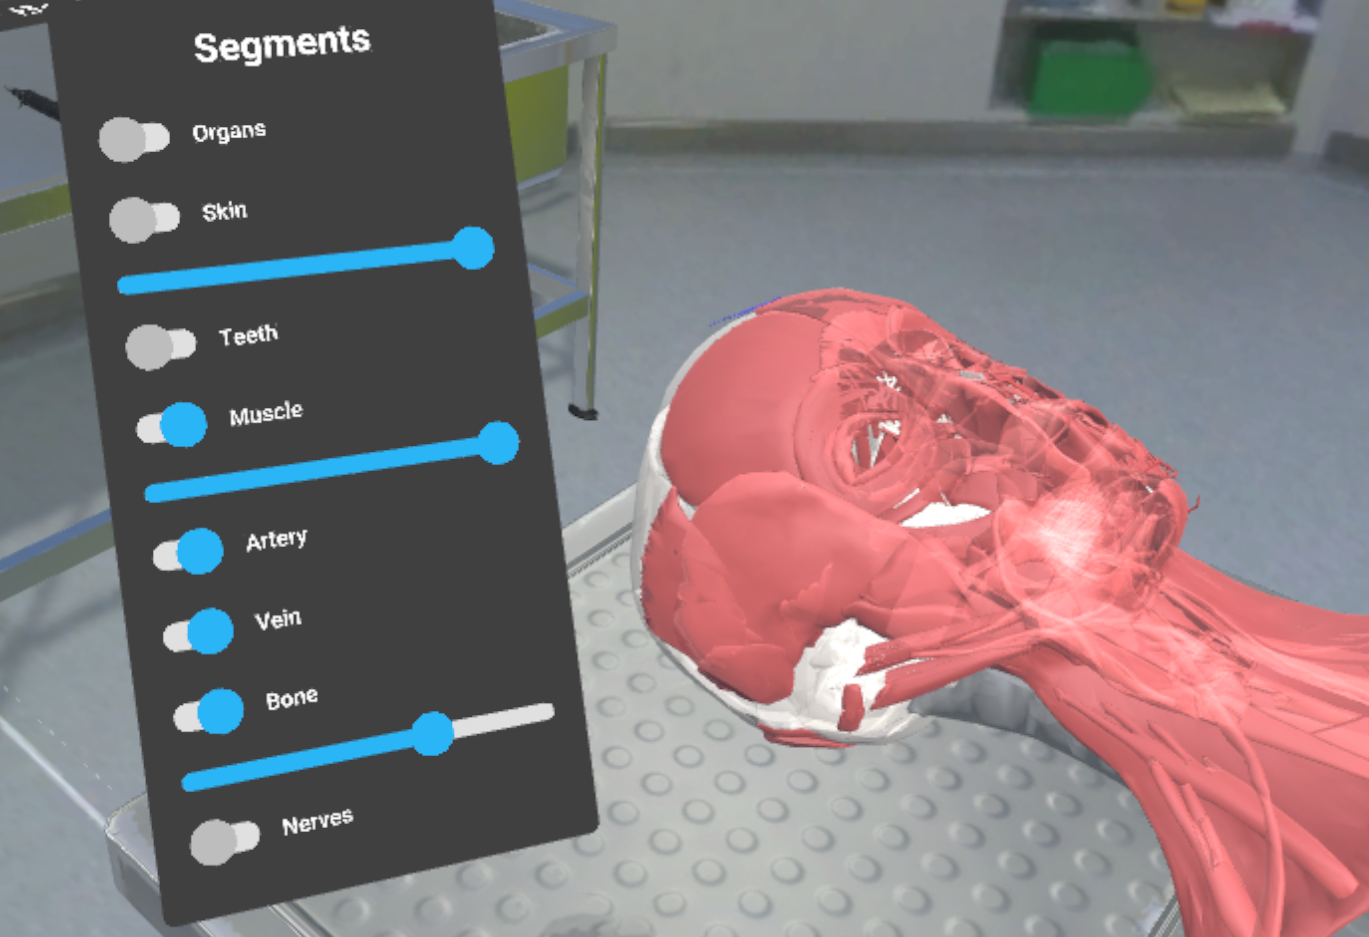
\includegraphics[width=0.95\linewidth]{images/implementation/features/visualization/segments_1.png}
  \end{minipage}%
  \begin{minipage}{.5\textwidth}
    \centering
    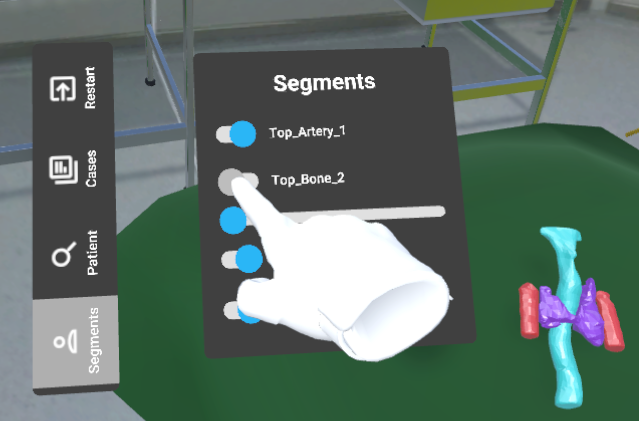
\includegraphics[width=0.915\linewidth]{images/implementation/features/visualization/segments_2.png}
  \end{minipage}
  \caption{\label{fig::Segmentation}Visualization - Segmentation}
\end{figure}

In Figure \ref{fig::Segmentation}, the process of activating and deactivating specific segments is described.
Users can also decide to adjust the transparency of segments as desired.

\begin{figure}[ht!]
    \centering
    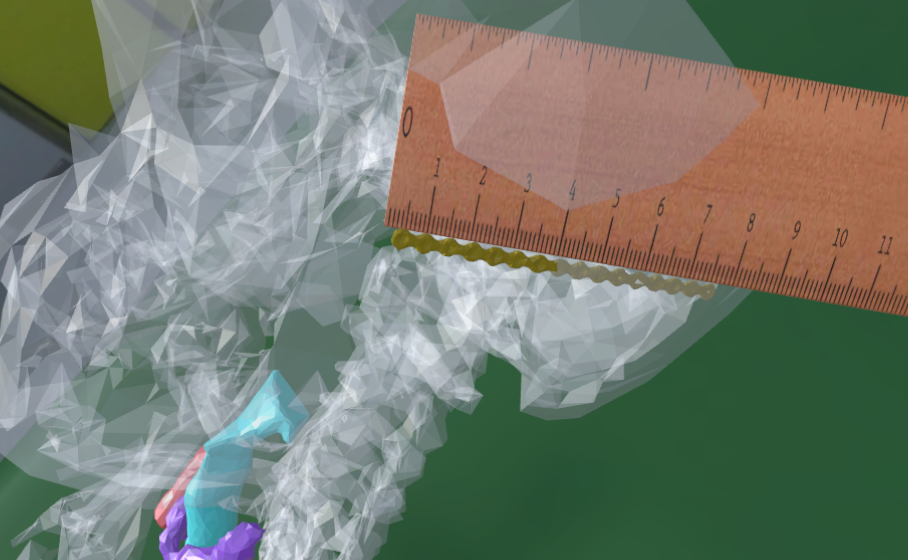
\includegraphics[width=\linewidth]{images/implementation/features/visualization/ruler.png}
    \caption{\label{fig::FeatureRuler} Ruler for Checking distances}
\end{figure}

\input{sections/4_implementation/features/visualization/explodeview.tex}